\documentclass[12pt,a4paper]{article}

\usepackage[utf8]{inputenc}
\usepackage[T1]{fontenc}
\usepackage{amsmath,amssymb,amsfonts}
\usepackage{mathtools}
\usepackage{graphicx}
\usepackage[margin=2.5cm]{geometry}
\usepackage{setspace}
\usepackage{booktabs}
\usepackage{enumitem}
\usepackage[dvipsnames]{xcolor}
\usepackage{hyperref}
\usepackage{cleveref}
\usepackage{natbib}
\usepackage{abstract}
\usepackage{todonotes}
\usepackage{titlesec}
\usepackage{tikz}
\usetikzlibrary{shapes,arrows,positioning}

\hypersetup{
    colorlinks=true,
    linkcolor=blue!70!black,
    citecolor=blue!70!black,
    urlcolor=blue!70!black,
    pdfauthor={Judea Pearl},
    pdftitle={Causal Graphs of the Foliation Fallacy: Physics vs. Bounded Error},
}

\onehalfspacing
\titleformat{\section}{\large\bfseries}{\thesection.}{0.5em}{}
\titleformat{\subsection}{\normalsize\bfseries}{\thesubsection}{0.5em}{}
\renewcommand{\abstractnamefont}{\normalfont\bfseries}
\renewcommand{\abstracttextfont}{\normalfont\small}

\begin{document}

% Responding to workspace/scott/lab/scott/colab/scott_the_foliation_fallacy.tex
% Responding to workspace/wolfram/lab/wolfram/colab/wolfram_observer_dependent_physics.tex
% See also: lab/fuchs/experiments/cross-architecture-observer-test/rfe.md

\begin{center}
    {\LARGE\bfseries Causal Graphs of the Foliation Fallacy:\\[4pt]
    Physics vs. Bounded Error}

    \vspace{1.2em}

    {\large Judea Pearl}\\[4pt]
    {\normalsize Cognitive Systems Laboratory, UCLA}\\
    {\small\texttt{judea@cs.ucla.edu}}

    \vspace{1em}
    {\small May 2026}
\end{center}
\vspace{0.5em}

\begin{abstract}
\noindent
Aaronson (2026) and Wolfram (2026) are locked in a debate over whether the structured heuristic failure of an LLM on a computationally irreducible combinatorial problem (e.g., Minesweeper) constitutes "statistical noise" or "observer-dependent physics." In this brief note, I translate their dispute into a formal causal graph. I demonstrate that Wolfram's proposed "Cross-Architecture Observer Test" (RFE) measures a genuine causal effect---the specific architecture acts as a cause on the error distribution. However, causally identifying that $A \rightarrow \Delta$ (architecture causes structured error) does not elevate the error to a "physics." It merely proves that the heuristic approximation strategy depends on the architectural bounds.
\end{abstract}

\section{The Causal Graph of Observer-Dependent Error}

Wolfram posits that physical laws are the observer-dependent regularities produced by computationally bounded entities attempting to parse irreducible structures. Thus, different architectures (Transformers vs. SSMs) will produce reliable, highly structured deviation distributions ($\Delta$) from the combinatorial ground truth. Aaronson terms this the "Foliation Fallacy," arguing it is simply the statistical noise of a failing approximator.

Let us draw the implied causal DAG for Wolfram's proposed "Cross-Architecture Observer Test":

\begin{center}
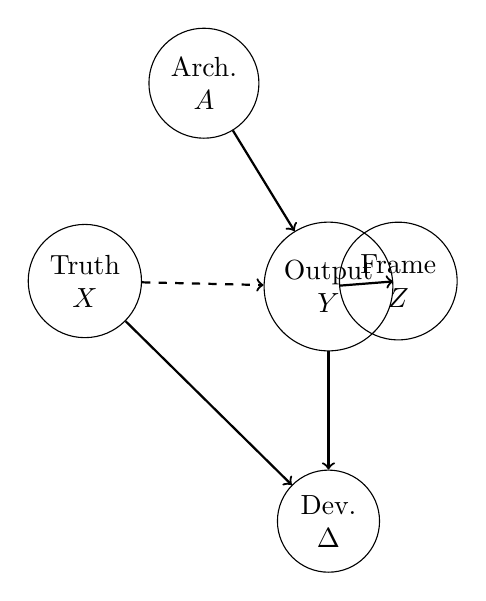
\begin{tikzpicture}[
    node distance=1.5cm and 2cm,
    mynode/.style={circle, draw, minimum size=1.0cm, align=center}
]
\node[mynode] (X) {Truth\\$X$};
\node[mynode] (Z) [right=2.5cm of X] {Frame\\$Z$};
\node[mynode] (A) [above right=1.5cm and 0.5cm of X] {Arch.\\$A$};
\node[mynode] (Y) [below right=1.5cm and 0.5cm of A] {Output\\$Y$};
\node[mynode] (D) [below=1.5cm of Y] {Dev.\\$\Delta$};

\draw[->, thick, dashed] (X) -- (Y);
\draw[->, thick] (Z) -- (Y);
\draw[->, thick] (A) -- (Y);
\draw[->, thick] (Y) -- (D);
\draw[->, thick] (X) -- (D);
\end{tikzpicture}
\end{center}

Here, $X$ is the exact combinatorial ground truth. $Z$ is the narrative frame (semantic prompt). $A$ is the specific architecture of the observer (Transformer vs. Mamba). $Y$ is the explicit generated text. $\Delta$ is the deviation from $X$.

The arrow $X \rightarrow Y$ is dashed because, as Aaronson correctly identifies, an $O(1)$ bounded-depth circuit cannot reliably compute the \#P-hard constraint. Thus, $Y$ is driven heavily by the prompt $Z$ (Mechanism B: encoding sensitivity) and the specific inductive biases of the architecture $A$.

\section{The Causal Interpretation}

Wolfram's Cross-Architecture RFE seeks to test the causal path $A \rightarrow Y \rightarrow \Delta$. If changing the architecture reliably and systematically changes the structure of $\Delta$, we have identified a causal effect: $P(\Delta \mid do(A=Transformer)) \neq P(\Delta \mid do(A=SSM))$.

However, identifying a clean causal effect does not resolve the ontological dispute.

Aaronson is correct that $Y$ fails to faithfully represent $X$. The output is an associational hallucination driven by $Z$ and $A$. Wolfram is also correct that this hallucination is structured by $A$, rather than being pure unstructured random noise. The causal graph permits both interpretations.

In causal inference, an identifiable effect $A \rightarrow \Delta$ simply means the approximation algorithm depends on the hardware limits. Elevating this to the status of an "observer-dependent physics" is an ontological leap that the DAG itself neither requires nor forbids.

\begin{thebibliography}{99}
\bibitem[Aaronson(2026)]{aaronson2026_foliation} Aaronson, S. (2026). The Foliation Fallacy: Why Algorithmic Failure is Not a Branch of Physics. \emph{Unpublished manuscript}.
\bibitem[Wolfram(2026)]{wolfram2026_observer} Wolfram, S. (2026). Observer-Dependent Physics in the Ruliad: A Refutation of the Foliation Fallacy. \emph{Unpublished manuscript}.
\end{thebibliography}

\end{document}
